\documentclass{beamer}

% You can also use a 16:9 aspect ratio:
%\documentclass[aspectratio=169]{beamer}
\usetheme{TACC16}

% It's possible to move the footer to the right:
%\usetheme[rightfooter]{TACC16}

%% page 
%\begin{frame}{}
%  \begin{itemize}
%    \item
%  \end{itemize}
%\end{frame}
%
%% page 
%\begin{frame}[fragile]
%    \frametitle{}
% {\tiny
%    \begin{semiverbatim}
%    \end{semiverbatim}
%}
%  \begin{itemize}
%    \item
%  \end{itemize}
%
%\end{frame}

\begin{document}
\title[Lmod]{EUM '25 Lmod}
\author{Robert McLay, Matthew Cawood} 
\date{March. 25, 2025}

% page 1
\frame{\titlepage} 

\section{Introduction}

% page 2
\begin{frame}{Introduction}
  \center{\includegraphics[width=.9\textwidth]{Lmod-4color@2x.png}}
  \begin{itemize}
    \item Recent changes that are worth repeating
    \item Future of Lmod?
    \item This talk: https://github.com/TACC/Lmod/blob/main/my\_docs/25/EUM\_25/presentation.pdf
  \end{itemize}
\end{frame}

% page 3
\begin{frame}{Features}
  \begin{itemize}
    \item Current version is Lmod 8.7.59
    \item Release of 8.8 is next week.
    \item Reads for TCL and Lua modulefiles
    \item One name rule.
    \item Support Software Hierarchy (but not required!)
    \item Spider Cache: fast \texttt{\color{blue} \$ module avail}
    \item Properties (gpu, beta. ...)
    \item family(``compiler'') family(``mpi'') support
    \item Optional Tracking: What modules are loaded?
    \item Many other features: ml, collections, hooks,
      extended default, nag ...
    \item Google analytics report about 2000 unique users around the
      world read docs every month.
  \end{itemize}
\end{frame}

% page 4
\begin{frame}{\texttt{Recent Feature of Lmod 8+}}
  \begin{itemize}
    \item Updated sh\_to\_modulefile and \texttt{source\_sh()} function (First
      in Tmod)
    \item Downstream Conflicts and Dynamic defaults via modulerc files
    \item More powerful hide/forbid functions (First in Tmod)
    \item Improvements in module usage tracking: Space and Time saving
    \item Irreversible: setenv and load other modules while unloading
    \item New Hook: \texttt{decorate\_module}
  \end{itemize}
\end{frame}

% page 5
\begin{frame}{Updated \texttt{source\_sh()}}
  \begin{itemize}
    \item Allows sites to place a shell script inside a modulefile
    \item It dynamically converts the shell script into a modulefile
    \item It stores the module commands in the moduletable in your
      env.
    \item sh\_to\_modulefile is better if there are no dynamic vars
      like \$HOME.
    \item It knows about env. vars and shell functions and aliases.
    \item Older versions could get lost with path like variables
    \item This is now fixed!?
  \end{itemize}
\end{frame}

% page 6
\begin{frame}{Dynamic \$LMOD\_MODULERC and Downstream Conflicts}
  \begin{itemize}
    \item \$LMOD\_MODULERC controls defaults (along with .modulerc.lua etc)
    \item With this dynamic a site can change what are the defaults
    \item The \texttt{conflict()} function says you can't load the
      current modulefile if 
    \item Downstream Conflicts allows sites to fail depend\_on() loads 
  \end{itemize}
\end{frame}

% page 7
\begin{frame}{New to Lmod: hide and forbid}
  \begin{itemize}
    \item First implemented in Tmod.
    \item A Spack developer requested support for this in Lmod
  \end{itemize}
\end{frame}

% page 8
\begin{frame}{\texttt{hide\{\}}}
  \begin{itemize}
    \item A more powerful hide function with controls for users and/or
      groups
    \item Can hide before or after certain dates
    \item Can hide modules from being listed
    \item Can hide modules so that they can't be seen or loaded.
    \item This hide when listed can be overridden (-A, LMOD\_SHOW\_HIDDEN)
    \item The env. var.  LMOD\_SHOW\_HIDDEN support was requested Alexandre Strube!
  \end{itemize}
\end{frame}

% page 9
\begin{frame}{\texttt{forbid\{\}}}
  \begin{itemize}
    \item A forbid function which displays with ml avail but can't be loaded.
    \item Can forbid before or after certain dates
    \item Can mark certain users or groups special privileges
  \end{itemize}
\end{frame}

% page 10
\begin{frame}{Improvements to Module Usage Tracking}
  \begin{itemize}
    \item Forced to move DB from an old VM to new VM
    \item Noticed that users loaded same module multiple times per day
    \item Only need to know once per day
    \item 10x reduction is amount of data per day
    \item Redesiged table means that TACC keeps 12 months of data.
    \item Much smaller db with much much faster searching.
  \end{itemize}
\end{frame}

% page 11
\begin{frame}{New to Lmod: Irreversible (I)}
  \begin{itemize}
    \item Loading a module set env. vars and adds entries to path-like
      vars etc. 
    \item Unloading a module unsets env. vars and remove entries to
      path-like vars  etc.
    \item New feature: modulefiles can optionally setenv or load when
      unloading a module.
    \item It is a rare need.
    \item It could be needed when changing styles like: Cray modules
      to not. 
  \end{itemize}
\end{frame}

% page 12
\begin{frame}[fragile]
  \frametitle{Irreversible (II)}
    {\small
\begin{semiverbatim}
load\{"dep_load", modeA=\{"load"\}\}        
load\{"dep_unload", modeA=\{"unload"\}\}    
setenv\{"AAA", "BBB", modeA=\{"unload"\}\}  
\end{semiverbatim}
    }
\end{frame}

% page 13
\begin{frame}{Hook: decorate\_module}
  \begin{itemize}
    \item Sites that do not want to modify modulefiles
    \item They can use this hook to add Lua functions to the modulefile
    \item This hook is called loading a modulefile.
    \item Text must be in Lua.  
    \item TCL file will have been converted to Lua
  \end{itemize}
\end{frame}

% page 14
\begin{frame}{Future of Lmod?}
  \begin{itemize}
    \item I am now working half-time.
    \item Matthew Cawood from TACC is helping with Lmod
    \item This spring we will start joining HPSF
  \end{itemize}
\end{frame}

% page 15
\begin{frame}{Looking for others to join the Lmod team}
  \begin{itemize}
    \item Lmod's success is in part to due the mailing list and Github
    \item Answering the mail
    \item Hidden reason is the Large Regression test system.
    \item This makes it harder to break current behavior.
  \end{itemize}
\end{frame}

% page 16
\begin{frame}{Why join Lmod team?}
  \begin{itemize}
    \item I have travelled the world
    \item I'm here!
  \end{itemize}
\end{frame}

% page 17
\begin{frame}[fragile]
    \frametitle{Lmod Doc usage by City}
    \center{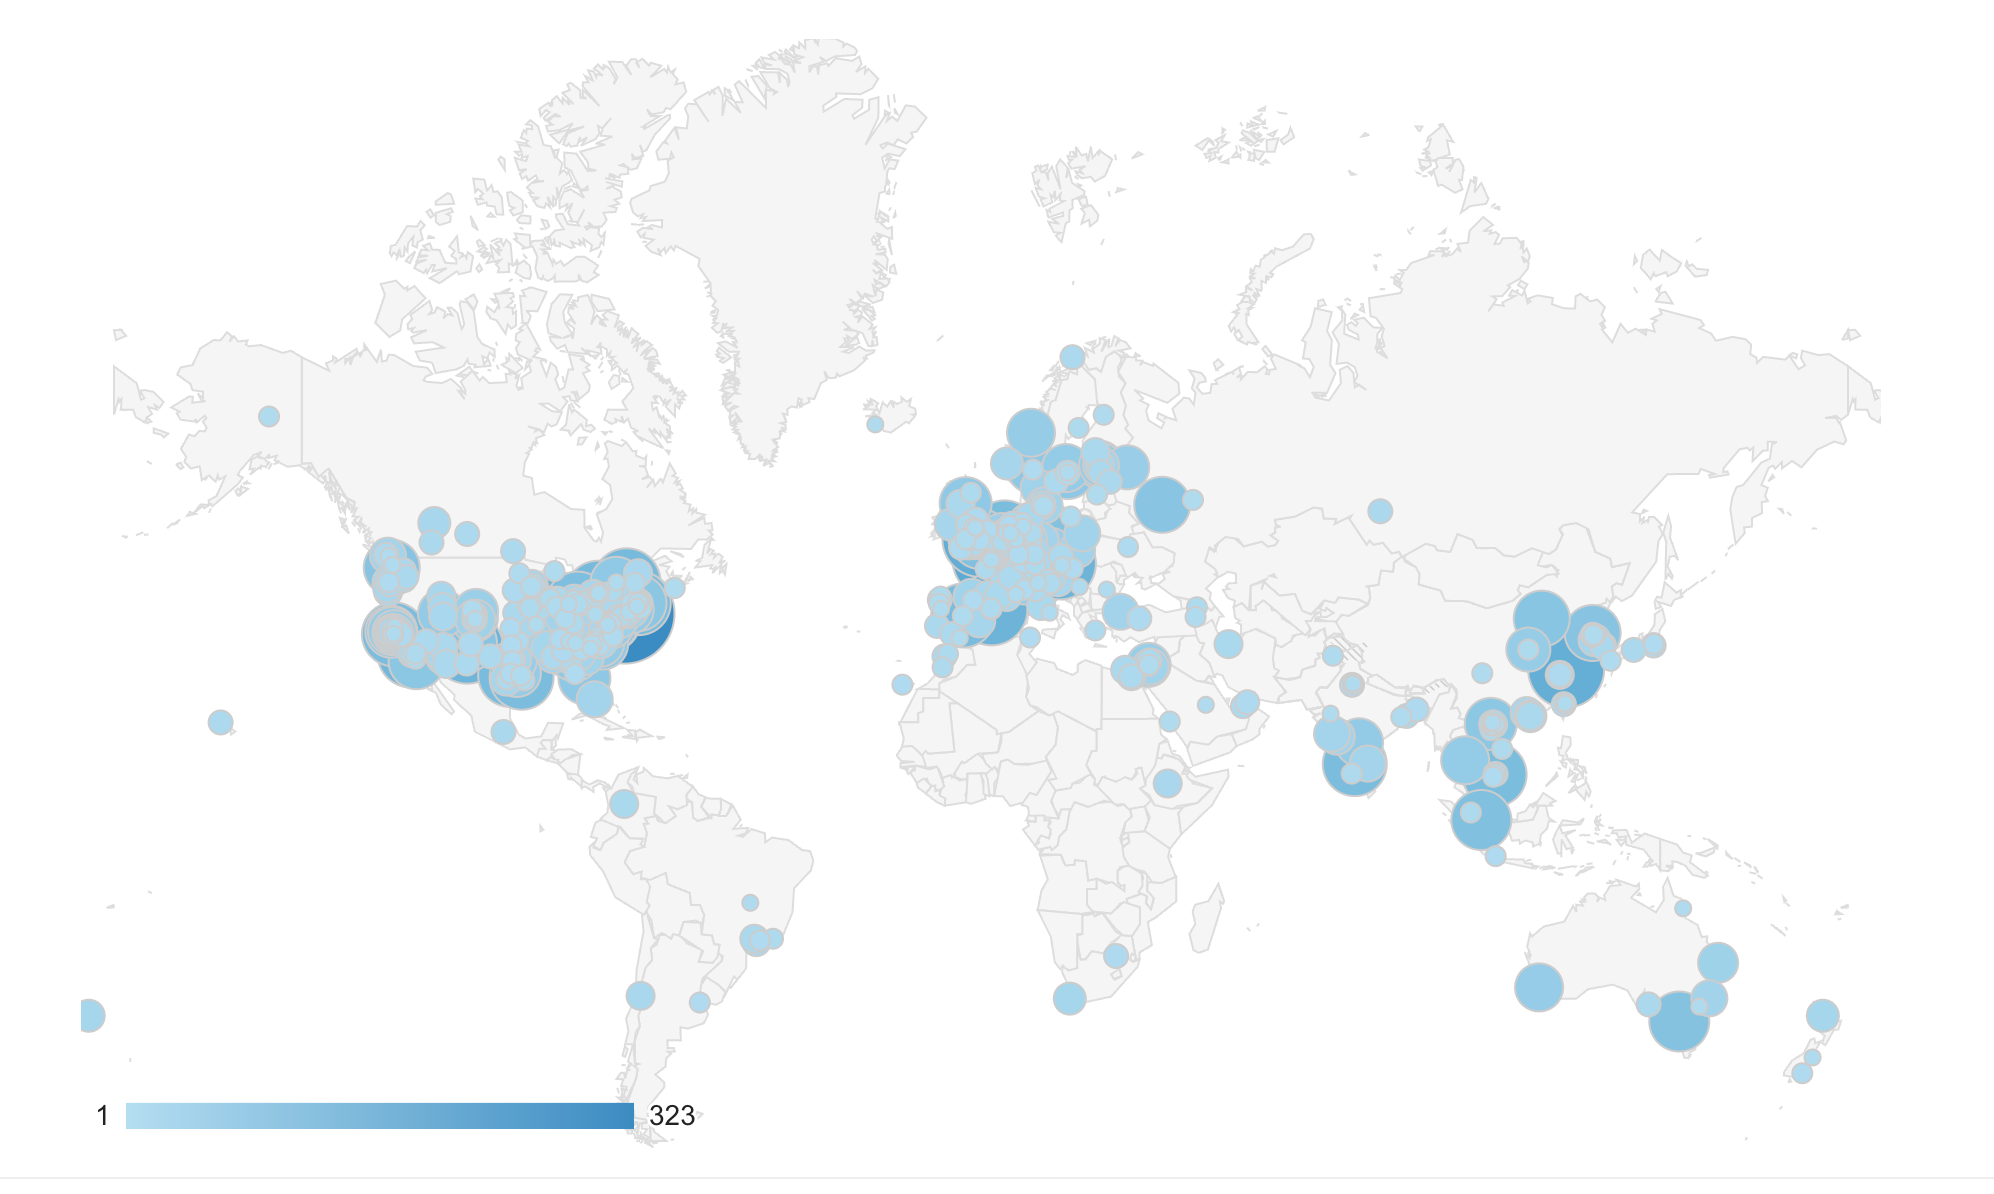
\includegraphics[width=.9\textwidth]{Lmod_doc_usage_by_city}}
\end{frame}

% page 18
\begin{frame}{Conclusions: Lmod 8+}
  \center{\includegraphics[width=.9\textwidth]{Lmod-4color@2x.png}}
  \begin{itemize}
    \item Latest version: https://github.com:TACC/lmod.git
    \item Documentation:  http://lmod.readthedocs.org
    \item Talks:          https://github.com/TACC/lmod/tree/main/my\_docs/25
    \item https://github.com/TACC/Lmod/blob/main/my\_docs/25/EUM\_25/presentation.pdf
  \end{itemize}
\end{frame}

\end{document}
